
\begin{frame}{Rewiring anisotropic networks}
  %
  \vspace{-0.8cm}
  \begin{columns}
    % 
    \begin{column}{.5\textwidth}
      \minipage[c][0.45\textheight][s]{\columnwidth}

      \begin{figure}
        \centering
        \includegraphics<1-3>[width=0.925\textwidth]{%
          figures/fig2AD_network_1cell_targets_158-aniso.png} %
        \includegraphics<4->[width=0.925\textwidth]{%
          figures/fig2AD_network_1cell_targets_158-rew.png} %
      \end{figure}
      
      
      
      \endminipage      
    \end{column}
    % 
    \begin{column}{.5\textwidth}
      \minipage[c][0.45\textheight][s]{\columnwidth}

      \vspace{0.2cm}
      
      \begin{center}
      \only<2>{\begin{overpic}[width=0.87\textwidth, frame=1pt]{%
            figures/figE.pdf}
      \end{overpic}}
      \only<3-4>{\begin{overpic}[width=0.87\textwidth, frame=1pt]{%
            figures/figF.pdf}
        \end{overpic}}

      \only<5>{\vspace{0.5cm}\begin{overpic}[width=\textwidth]{%
            figures/netw_dist-dep_aniso-rew.pdf}
        \end{overpic}}      

      \end{center}
      
      \endminipage
    \end{column}
  \end{columns}

  % \vspace{-0.6cm}
  
  % \begin{columns}
  %   % 
  %   \begin{column}{.5\textwidth}
  %     \minipage[c][0.25\textheight][s]{\columnwidth}

  %     \begin{figure}
  %       \centering
  %       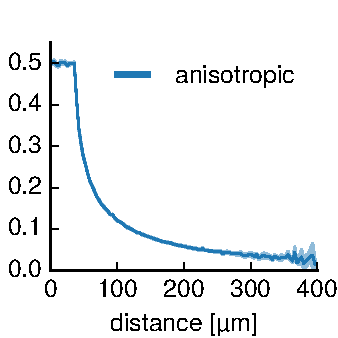
\includegraphics[width=0.8\textwidth]{%
  %         figures/netw_dist-dep_aniso.pdf} %
  %     \end{figure}

      
      
  %     \endminipage      
  %   \end{column}
  %   % 
  %   \begin{column}{.5\textwidth}
  %     \minipage[c][0.25\textheight][s]{\columnwidth}

  %     \begin{figure}
  %       \centering
  %       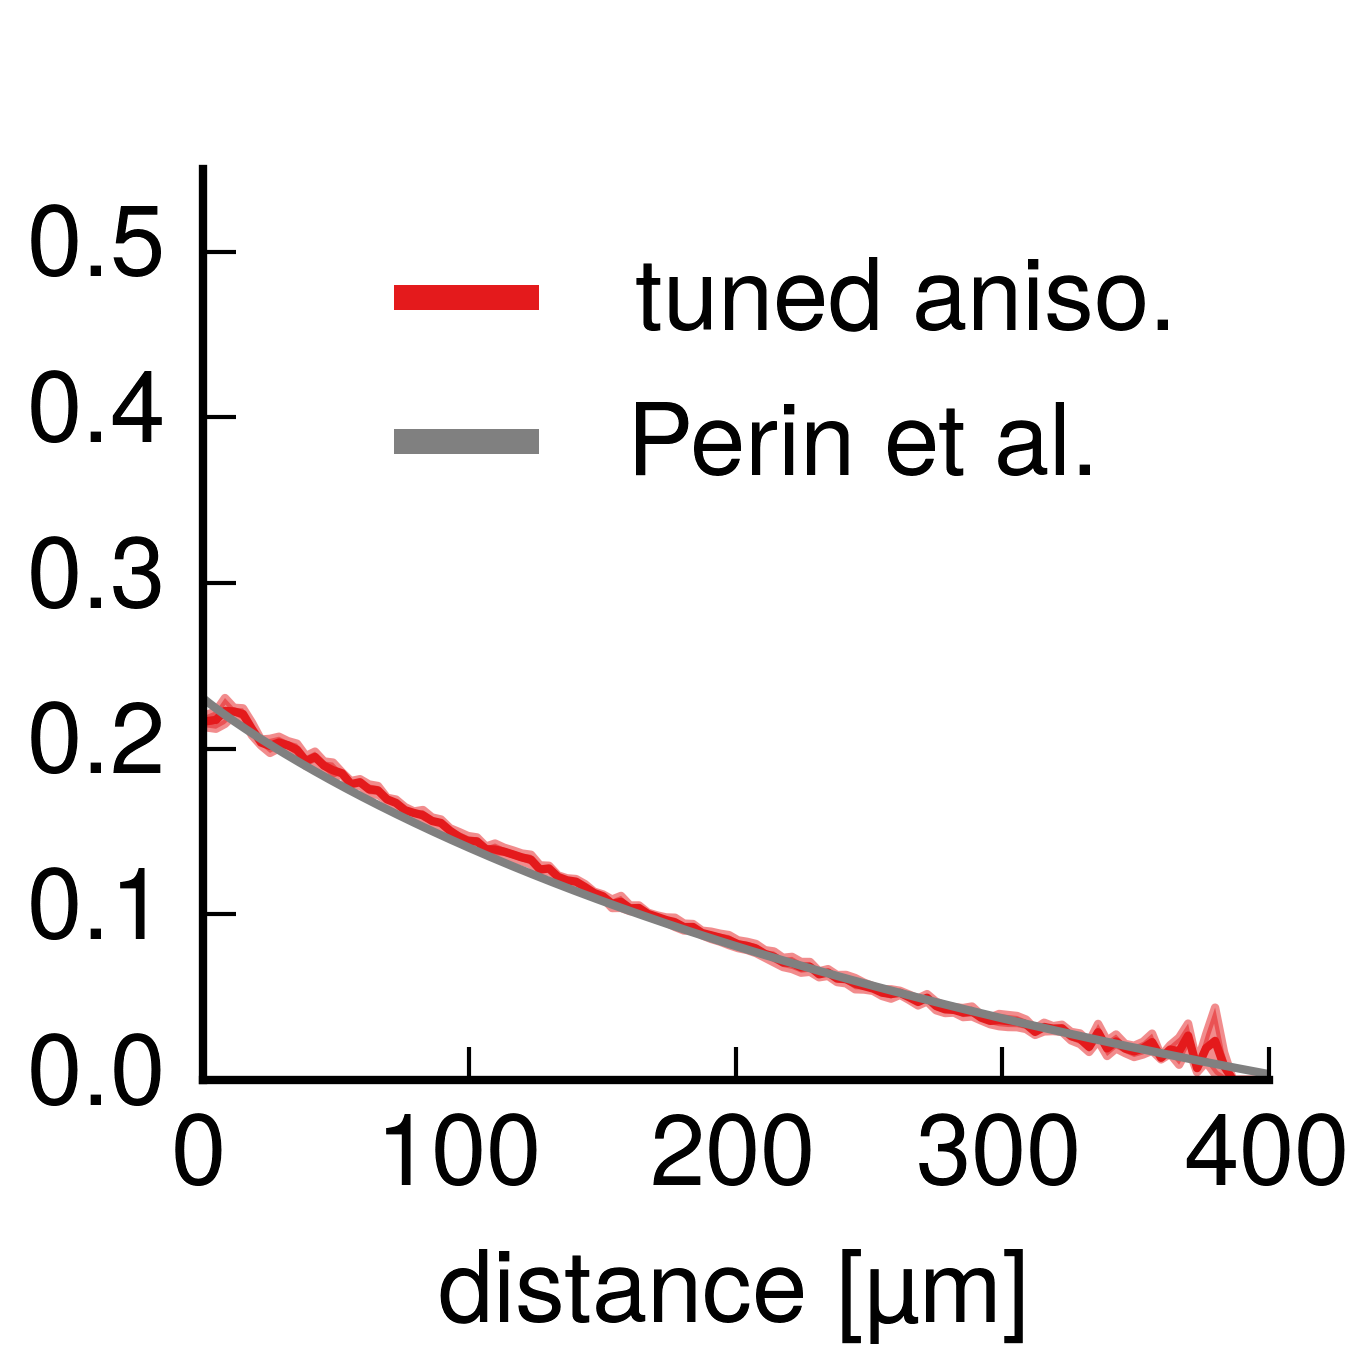
\includegraphics[width=0.8\textwidth]{%
  %         figures/fig2H_tuned-aniso-ddcp.png} %
  %     \end{figure}

      
      
  %     \endminipage      
      
      
  %   \end{column}
  % \end{columns}
  


  
\end{frame}





